%% storify: covariate-artifact correction, the whole counterfactual testbed, written for an
%% external reviewer (rewrite of 2026-11-04). The PI lifted the page and word caps for this
%% paper. Edit THIS file. Run `python3 build_story.py` to write story.tex, then
%% `latexmk -pdf story.tex`. Never edit story.tex by hand: the build overwrites it.
%%
%% numbers   every measured number is a macro that the build defines in the data slot below.
%% typed     design constants only, each in \lit{}: 25 bp and 1 kb bins; 30M and 50M original
%%           depths; 15M, 7.5M and 3.75M depth versions; 36 and 50 bp crops; MAPQ 10 and 0;
%%           antibody proxy 50% and 90% control reads; fragment-extension and control-scaling
%%           factors 0.5 and 2; control depth 50% and 25%; chr19, chr21, chr22; 3 and 6 seeds;
%%           2 x seed range; log2 and log10; 40 signal-level bins; top 1% of bins; 36-mer
%%           mappability; 5 Mb shift; objective weights 1 and 4; 0.5 gap-closed threshold;
%%           0.10 and 0.16 depth-rule limits; CRPS 20 divergence limit; histone mark names
%%           (H3K27ac, H3K4me1, H3K4me3, H3K27me3, H3K36me3, H3K9me3); the 12 cells per form.
\documentclass[pdflatex,sn-mathphys-num]{sn-jnl}

% crux-sources: {"h29_adding_a_cross_assay_imputation_or_maske.md": "0fa755e3b02fa1f02698ea63f2e87b34d075a2f42155d91f4cd72a98b39a1838", "h30_chaining_one_shared_count_space_correcti.md": "81f792f6a60c33cbd389e06e995477dbaa2485c427c4288682cfa6548d34c7c8", "h31_giving_the_shared_count_space_correction.md": "ec7b3ad38869928ec5b055f5d77d6cb6088c9c3cff71ab2d11e5bc8465fddc91", "notes/mini_candi_design_inputs.md": "485a6bf615e94e2af9e1bd37a34444a61cde8d76fb37090c28cad2eddb0504fa", "q1_do_the_recorded_experimental_covariates_.md": "7f2c5b7422eefde2670f3e1223fea707be31a21c8f9a21c2af552ce17395b47a", "results/h12/checks_A.json": "ba2e61d607fd220c18183428a7fa866298223c5f518217263e80b4f1ca68bcbf", "results/h12/report.md": "6819211f9d4cdc9bf686bafbe056a195a70fac060be64a90107d2429dc141c0f", "results/h13/checks_C.json": "59a7d9c236a41e7f7341d422ffe6ad814f263c9c1eb18bfb38e5af083d8abb2d", "results/h13/report.md": "6a6abf440d773a94102bdf1524d8426eb5ebeef46b5609f0677910c0f73002d9", "results/h14/checks_D.json": "756d307a9b8270bf5ff816575ce7c78cf01f03f57be47938a38a5147de58da2c", "results/h14/report.md": "4d6718ab134d91a7105e49544759890842127238d50d3e21b84c2d35f974cd85", "results/h15/report.md": "1a627c961d3e0204db7eb34de5744e566f36dcc62a5572564784e6f79785cb02", "results/h17/checks_B.json": "b2ad3fe45f675a3190ef487e463fa04e4f0fa20f41c49cecbf14804bf9feb57d", "results/h17/report.md": "e9a99dac5533c7349dabae4e0bffc0d8bbb030c827f36f53ed335571353404ab", "results/h19/depth_pairs/compose_out.txt": "996f5c35f0b076dfcf8d95d2767a23a745ed65db19ba6513f0d569c37c37bf05", "results/h19/knob_generalization/depth_table.tsv": "03bcad2ad70603c5be735287a7e5374fde8c77344f091aaeb83efef71abf6380", "results/h19/knob_generalization/group_table.tsv": "2c0c89ae7409e736993ebfc05baf0d999f97fa78b5b2ca4396c746bc0338c5e5", "results/h19/knob_generalization/knob_table.tsv": "dbab28911a5a807e45a2d8fa00a3aaaf68f65e32fecc891d393b0b74280114fb", "results/h19/knob_generalization/verify.txt": "a29dfb5c0f41029547a8198253aadb9cc274daf0946ce1db8e757372deff0ead", "results/h26/results.json": "09d70318722324098b47be7f924b136edca4dcf7eccd7e305ad6d43723cc6800", "results/t122/AUDIT.md": "d137ae1c41217c54de7651644d14b527c49595c99e1902db453d5e92b66cc93c", "results/t125/h_alone_summary.tsv": "e572d440646bee7831c451245e0057ee36024e67f0269d8d0c879d87a8c382d2", "results/t125/h_vs_oldgrid.tsv": "bd72790869123e38524187dac6894d48f0e60ad97d3d57a92311c71be7f9c10e", "results/t125/part1_digest.md": "ad3e66d7aacd44101b02a386f728c95fe2c0af466c93e2a9428477cfb71aeea4", "results/t125/part2_digest.md": "953db8ff3884ecb22e16a643cd1ea9d84a8ba4d43b14b0bfc4935cf4d6648d5e", "results/t127/depth_law.csv": "3b6826b1922020d812ac309b0f93e889d3ea67c928b4436a286462fdff48ecbc", "results/t128/depth_table.tsv": "c61e99c71832eab736f3d4f1faa65db90364474fff065377740407025041588d", "results/t128p3/m1_never_table.tsv": "cd94fcde9d1f5456a4ceda4dead05fed07ea0f5a714951ef962083d2f36cd33e", "results/t128p3/m5_depthlaw_table.tsv": "269eec8f4046441c9a6dc21665a4325b5d25cc44c3879968407e3917388f1298", "results/t130/blind_table.tsv": "32c5f06704b0617120c5e76f5a26563b963bbb6d18cbbeaaf4b408fc6181907d", "results/t130/nested_dispersion.tsv": "895510f95be1b0f7d461d80384a4ab266fec9f2dcd6357c0767e1530562ddd31", "results/t133/ranking.tsv": "122653ae9e59a9687276515d913e5983e5266f7c745b8239db439510861e124e", "results/t136/checks_readings.tsv": "0877a71121c98e2de20f499924764c74d3f255be60001d21023d67965789d476", "results/t136/m1_heldout_table.tsv": "5875c5d515d0aab3c8add24e7bf5ee46b0a7ddf499e2722a0ceb608d0f3615e2", "results/t136/m5_depthlaw_table.tsv": "b91f57011d86e9f7521b002406d21d61e437d9a01796dba5ae5191c1f3cdc41c", "results/t137/floor_at_30M.tsv": "57c79b0fb27abb7455b3579b5fba3cf482254003af58ce42d885974dbf75e63c", "results/t138/map_classes.tsv": "0dbc2954ccf8c1b77c07fcd5dfb61ffcbefdfc0fa6f97c1cbd20e2b5f9f4a8d3", "results/t139/knob_vs_floor.tsv": "48e437cac296e22ef3ed9042c92f272376c43ef92c145a088ae0c9ec616a19a2", "results/t142/compare_real_class.tsv": "7ea9c6c29594be886f9fcaa933f41cd9a6fc55f00c36a355e50d031c214a03af", "results/t142/floor_at_30M.tsv": "2efdb6407090b8b8df6be6f60a15835561ef4b85ce1931a4521064c562a2d3b3", "results/t142/map_classes.tsv": "a5aa69c06e7ad58a5557e5cb814b9205ee40a9658f8183711d2ae35ebd5094b6", "results/t142/t141_readthin/knob_classes.tsv": "1ceeba1c40c989da90be8eb9b496de23010c69ff0108fa88211cad6ebfafa846", "results/t146/REPORT.md": "4065a7aa83bc1bc90c3c22742cdae83000edcaedb44507655198a6d87283a377", "results/t146/analyze_out.txt": "8b3b934ee8ae81813536746bd4a8e3b9a7d80b40900df806dfe9cf6085c92a31", "results/t146/checks_h29.tsv": "d17798ada1e9a3cec65cb044fedd23338430aae56755b89d91f5f70117d9ac48", "results/t146/checks_h29_pooled.tsv": "cfa93efc194413b657dfdd3bdd45aef48ea6a7453052f661d5809c89b67120af", "results/t146/checks_h30_cells.tsv": "14b5c615e208bc03d81aac8082aa7071a0043015b06f8a43ce7097d3cdecceac", "results/t146/checks_h30_pooled.tsv": "a835f651247727a17aee07aea31773aad8b486d95586bfa11923e3bef2de7217", "results/t146/checks_h31.tsv": "14ba8ae9a16816c1b98106d981ad34fed57cf0657df9d332410245e53eefab6b", "results/t146/checks_h31_per_track_seed.tsv": "5094b25a2b75163b883d41496ed6e0f87f1183e34bb7cbf1fbdd79092a6b5f60", "results/t146/depthlaw.tsv": "775ccd918cff1e533674ed5de7de12bf2f90f31c8c5500a79aee74be1e5f04a2", "results/t146/pooled.tsv": "98e6ecdc8300efad70c05143bfda0ae93d4716b4cd0fe7f9391615da67159949", "stories/q1/build_story.py": "715d291945fb0368fd803aaea78ec5a08421038ebccbfdfa66f8034ddce50516", "stories/q1/story_src.tex": "f744b8e7d4ed882939a42faf72fde4eab9e3e500f0e42cd7fc370f58765bfcef", "wiki/encode-imputation-challenge.md": "3b179980d35be86bc7bb3b03c13308164ece24554446bc7e1c1a63f03aa5b539"}

\usepackage{graphicx}
\usepackage{amsmath}
\usepackage{booktabs}
\usepackage{array}
\usepackage{xcolor}
\usepackage{tikz}
\usetikzlibrary{positioning,arrows.meta,calc,fit}
\usepackage{pgfplots}
\pgfplotsset{compat=1.18}
\usepackage{pgfplotstable}

% A design constant typed in prose, e.g. \lit{95}. It renders its argument unchanged.
\newcommand{\lit}[1]{#1}

% One colour per model form, per mark class and per CRPS part; defined once.
\definecolor{dA}{HTML}{9A9A9A}
\definecolor{dB}{HTML}{3F7D7A}
\definecolor{dC}{HTML}{B5462E}
\definecolor{dD}{HTML}{4B5FA6}
\definecolor{cDn}{HTML}{B5462E}
\definecolor{cNar}{HTML}{3F7D7A}
\definecolor{cBr}{HTML}{4B5FA6}
\definecolor{pOS}{HTML}{4B5FA6}
\definecolor{pSE}{HTML}{D9A441}
\definecolor{gTr}{HTML}{3F7D7A}
\definecolor{gNv}{HTML}{B5462E}
\definecolor{gCr}{HTML}{D9A441}

% shared chart styles
\pgfplotsset{
  base/.style={tick label style={font=\scriptsize}, label style={font=\footnotesize},
    title style={font=\footnotesize}, legend style={font=\scriptsize, draw=none, fill=white,
    fill opacity=0.8, text opacity=1}, legend cell align=left},
  stk/.style={base, ybar stacked, bar width=10pt, ymin=0, xtick=data,
    xticklabel style={rotate=30, anchor=north east, font=\scriptsize}, xtick style={draw=none},
    legend style={at={(0.02,0.98)}, anchor=north west}, area legend},
}

\newcommand{\armAllRule}{0.151}
\newcommand{\armAllRuleS}{0.028}
\newcommand{\armOneRule}{0.148}
\newcommand{\armOneRuleS}{0.123}
\newcommand{\armRefRule}{0.195}
\newcommand{\armRefRuleS}{0.061}
\newcommand{\armTwoAll}{21}
\newcommand{\armTwoDone}{21}
\newcommand{\armViaRule}{0.125}
\newcommand{\armViaRuleS}{0.022}
\newcommand{\bitsFull}{0.551}
\newcommand{\bitsPanel}{0.000}
\newcommand{\cFourBar}{0.125}
\newcommand{\cFourGain}{\ensuremath{-}0.048}
\newcommand{\cFourGainChk}{\ensuremath{-}0.048}
\newcommand{\cFourGap}{\ensuremath{-}0.53}
\newcommand{\cOneGap}{0.674}
\newcommand{\cThreeBar}{0.367}
\newcommand{\cThreeHeld}{0.148}
\newcommand{\cThreeTr}{0.120}
\newcommand{\cThreeTrS}{0.106}
\newcommand{\corpEic}{363}
\newcommand{\corpEicBio}{89}
\newcommand{\corpMerged}{3{,}026}
\newcommand{\corpMergedBio}{361}
\newcommand{\costBam}{1}
\newcommand{\costFastq}{13.4}
\newcommand{\costFastqMax}{30.6}
\newcommand{\costTrHi}{36}
\newcommand{\costTrLo}{11}
\newcommand{\crArm}{0.573}
\newcommand{\crArmOS}{0.466}
\newcommand{\crArmS}{0.062}
\newcommand{\crArmSE}{0.107}
\newcommand{\crArmTwo}{0.428}
\newcommand{\crArmTwoGap}{1.08}
\newcommand{\crArmTwoOS}{0.425}
\newcommand{\crArmTwoS}{0.005}
\newcommand{\crArmTwoSE}{0.003}
\newcommand{\crRef}{0.525}
\newcommand{\crRefOS}{0.473}
\newcommand{\crRefS}{0.032}
\newcommand{\crRefSE}{0.052}
\newcommand{\crVia}{0.435}
\newcommand{\crViaOS}{0.429}
\newcommand{\crViaS}{0.003}
\newcommand{\crViaSE}{0.006}
\newcommand{\cropFeatHi}{0.042}
\newcommand{\cropFeatLo}{0.013}
\newcommand{\ctlNoneHi}{0.077}
\newcommand{\ctlNoneLo}{0.063}
\newcommand{\ctlPSameHi}{0.48}
\newcommand{\ctlPSameLo}{0.31}
\newcommand{\ctlPTrHi}{0.62}
\newcommand{\ctlPTrLo}{0.36}
\newcommand{\ctlWobHi}{0.024}
\newcommand{\ctlWobLo}{0.003}
\newcommand{\dedupFeatHi}{0.0023}
\newcommand{\dedupFeatLo}{0.0005}
\newcommand{\depArm}{0.774}
\newcommand{\depArmFeatHi}{0.0032}
\newcommand{\depArmFeatLo}{0.0001}
\newcommand{\depNull}{0.773}
\newcommand{\depNullFeatHi}{0.0031}
\newcommand{\depNullFeatLo}{0.0002}
\newcommand{\dispHi}{1.005}
\newcommand{\dispLo}{0.994}
\newcommand{\dnA}{3.060}
\newcommand{\dnAOS}{1.360}
\newcommand{\dnAS}{0.113}
\newcommand{\dnASE}{1.700}
\newcommand{\dnB}{0.824}
\newcommand{\dnBOS}{0.816}
\newcommand{\dnBS}{0.004}
\newcommand{\dnBSE}{0.007}
\newcommand{\dnC}{0.818}
\newcommand{\dnCOS}{0.802}
\newcommand{\dnCS}{0.027}
\newcommand{\dnCSE}{0.016}
\newcommand{\dnD}{0.772}
\newcommand{\dnDOS}{0.760}
\newcommand{\dnDS}{0.036}
\newcommand{\dnDSE}{0.012}
\newcommand{\dnaShareHi}{0.29}
\newcommand{\dnaShareLo}{0.21}
\newcommand{\featLowUnit}{0.008}
\newcommand{\featMax}{0.0003}
\newcommand{\featMaxFifteen}{0.0003}
\newcommand{\fitArm}{0.063}
\newcommand{\fitArmS}{0.008}
\newcommand{\fitRef}{0.052}
\newcommand{\fitRefS}{0.010}
\newcommand{\fixNeverHi}{0.63}
\newcommand{\fixNeverLo}{0.28}
\newcommand{\fixTrHi}{0.12}
\newcommand{\fixTrLo}{0.05}
\newcommand{\floorCtxHi}{0.40}
\newcommand{\floorCtxLo}{0.36}
\newcommand{\floorFeatHi}{0.00009}
\newcommand{\floorFeatLo}{0.00002}
\newcommand{\gAl}{0.660}
\newcommand{\gAlOS}{0.610}
\newcommand{\gAlS}{0.031}
\newcommand{\gAlSE}{0.050}
\newcommand{\gMap}{0.665}
\newcommand{\gMapOS}{0.605}
\newcommand{\gMapS}{0.011}
\newcommand{\gMapSE}{0.060}
\newcommand{\gcAHi}{\ensuremath{-}0.01}
\newcommand{\gcALo}{\ensuremath{-}0.62}
\newcommand{\gcAnoiseHi}{2.6}
\newcommand{\gcAnoiseLo}{0.7}
\newcommand{\gcBDHi}{0.92}
\newcommand{\gcBDLo}{0.77}
\newcommand{\gcBDnoiseHi}{0.53}
\newcommand{\gcBDnoiseLo}{0.02}
\newcommand{\gcCDabHi}{3.68}
\newcommand{\gcCDabLo}{1.11}
\newcommand{\genCropSame}{0.05}
\newcommand{\genCropTr}{0.18}
\newcommand{\genDepthHi}{0.46}
\newcommand{\genDepthLo}{0.16}
\newcommand{\genDepthSame}{0.16}
\newcommand{\genDepthTr}{0.46}
\newcommand{\hAff}{0.1791}
\newcommand{\hAffOS}{0.1367}
\newcommand{\hAffSE}{0.0423}
\newcommand{\hAffW}{0.0010}
\newcommand{\hBest}{0.0659}
\newcommand{\hBestOS}{0.0656}
\newcommand{\hBestSE}{0.0003}
\newcommand{\hBestW}{0.0035}
\newcommand{\ivBHi}{0.031}
\newcommand{\ivBLo}{0.028}
\newcommand{\jAlone}{0.667}
\newcommand{\jAloneOS}{0.612}
\newcommand{\jAloneS}{0.019}
\newcommand{\jAloneSE}{0.055}
\newcommand{\jDn}{0.674}
\newcommand{\jDnOS}{0.629}
\newcommand{\jDnS}{0.051}
\newcommand{\jDnSE}{0.045}
\newcommand{\jDnd}{\ensuremath{+}0.007}
\newcommand{\jDndBar}{0.103}
\newcommand{\jDndSE}{\ensuremath{-}0.010}
\newcommand{\jDnids}{0.956}
\newcommand{\jDnidsOS}{0.697}
\newcommand{\jDnidsS}{0.041}
\newcommand{\jDnidsSE}{0.259}
\newcommand{\jDnnw}{\ensuremath{-}0.009}
\newcommand{\jDnnwBar}{0.094}
\newcommand{\jDnnwSE}{\ensuremath{-}0.011}
\newcommand{\jDntw}{\ensuremath{+}0.282}
\newcommand{\jDntwBar}{0.103}
\newcommand{\jMatch}{0.659}
\newcommand{\jMatchOS}{0.613}
\newcommand{\jMatchS}{0.017}
\newcommand{\jMatchSE}{0.047}
\newcommand{\jX}{0.642}
\newcommand{\jXOS}{0.603}
\newcommand{\jXS}{0.034}
\newcommand{\jXSE}{0.039}
\newcommand{\jXd}{\ensuremath{-}0.025}
\newcommand{\jXdBar}{0.067}
\newcommand{\jXdSE}{\ensuremath{-}0.016}
\newcommand{\jXfour}{0.633}
\newcommand{\jXfourOS}{0.607}
\newcommand{\jXfourS}{0.014}
\newcommand{\jXfourSE}{0.026}
\newcommand{\jXfourd}{\ensuremath{-}0.034}
\newcommand{\jXfourdBar}{0.039}
\newcommand{\jXfourdSE}{\ensuremath{-}0.029}
\newcommand{\jXids}{0.964}
\newcommand{\jXidsOS}{0.692}
\newcommand{\jXidsS}{0.034}
\newcommand{\jXidsSE}{0.271}
\newcommand{\jXnw}{\ensuremath{-}0.005}
\newcommand{\jXnwBar}{0.124}
\newcommand{\jXnwSE}{\ensuremath{-}0.009}
\newcommand{\jXtw}{\ensuremath{+}0.322}
\newcommand{\jXtwBar}{0.068}
\newcommand{\knobShufHi}{0.00001}
\newcommand{\knobShufLo}{0.00000}
\newcommand{\knobShufMax}{0.00003}
\newcommand{\lDnaL}{\ensuremath{+}0.015}
\newcommand{\lDnaLBar}{0.006}
\newcommand{\lDnaQ}{\ensuremath{+}0.011}
\newcommand{\lDnaQBar}{0.006}
\newcommand{\lMapL}{\ensuremath{+}0.045}
\newcommand{\lMapLBar}{0.005}
\newcommand{\lMapQ}{\ensuremath{+}0.051}
\newcommand{\lMapQBar}{0.003}
\newcommand{\lawArm}{0.148}
\newcommand{\lawArmS}{0.123}
\newcommand{\lawData}{0.71}
\newcommand{\lawNeverAllHi}{0.63}
\newcommand{\lawNeverAllLo}{0.24}
\newcommand{\lawRef}{0.195}
\newcommand{\lawRefS}{0.061}
\newcommand{\lawSeedHi}{0.213}
\newcommand{\lawSeedLo}{0.089}
\newcommand{\lawTrAllHi}{0.12}
\newcommand{\lawTrAllLo}{0.05}
\newcommand{\lawVia}{0.125}
\newcommand{\lawViaAllHi}{0.11}
\newcommand{\lawViaAllLo}{0.09}
\newcommand{\lawViaS}{0.022}
\newcommand{\lvlFifteenHi}{0.38}
\newcommand{\lvlFifteenLo}{0.18}
\newcommand{\lvlLowHi}{0.32}
\newcommand{\lvlLowLo}{0.21}
\newcommand{\mAlL}{0.353}
\newcommand{\mAlLOS}{0.322}
\newcommand{\mAlLS}{0.004}
\newcommand{\mAlLSE}{0.031}
\newcommand{\mAlQ}{0.590}
\newcommand{\mAlQOS}{0.569}
\newcommand{\mAlQS}{0.004}
\newcommand{\mAlQSE}{0.020}
\newcommand{\mDedupChg}{\ensuremath{-}0.0166}
\newcommand{\mDepthChg}{\ensuremath{-}0.0094}
\newcommand{\mDepthSD}{0.0011}
\newcommand{\mDnaL}{0.338}
\newcommand{\mDnaLOS}{0.316}
\newcommand{\mDnaLS}{0.011}
\newcommand{\mDnaLSE}{0.022}
\newcommand{\mDnaQ}{0.577}
\newcommand{\mDnaQOS}{0.558}
\newcommand{\mDnaQS}{0.011}
\newcommand{\mDnaQSE}{0.020}
\newcommand{\mGainL}{\ensuremath{+}0.050}
\newcommand{\mGainQ}{\ensuremath{+}0.057}
\newcommand{\mMapL}{0.303}
\newcommand{\mMapLOS}{0.300}
\newcommand{\mMapLS}{0.010}
\newcommand{\mMapLSE}{0.003}
\newcommand{\mMapQ}{0.532}
\newcommand{\mMapQOS}{0.530}
\newcommand{\mMapQS}{0.004}
\newcommand{\mMapQSE}{0.002}
\newcommand{\mShL}{0.348}
\newcommand{\mShLOS}{0.323}
\newcommand{\mShLS}{0.006}
\newcommand{\mShLSE}{0.026}
\newcommand{\mShQ}{0.594}
\newcommand{\mShQOS}{0.573}
\newcommand{\mShQS}{0.004}
\newcommand{\mShQSE}{0.021}
\newcommand{\mapqZeroDecAllHi}{0.48}
\newcommand{\mapqZeroDecAllLo}{0.45}
\newcommand{\mapqZeroDecHi}{0.48}
\newcommand{\mapqZeroDecLo}{0.45}
\newcommand{\mapqZeroHi}{0.110}
\newcommand{\mapqZeroLo}{0.099}
\newcommand{\nArmsDisp}{21}
\newcommand{\nBDcells}{18}
\newcommand{\nBDgain}{18}
\newcommand{\nBlA}{--}
\newcommand{\nBlB}{9}
\newcommand{\nBlC}{5}
\newcommand{\nBlD}{1}
\newcommand{\nCellNeed}{66}
\newcommand{\nCellWin}{2}
\newcommand{\nCellWorse}{0}
\newcommand{\nCells}{98}
\newcommand{\nCellsA}{12}
\newcommand{\nCellsB}{12}
\newcommand{\nCellsC}{12}
\newcommand{\nCellsD}{12}
\newcommand{\nCfg}{16}
\newcommand{\nCross}{90}
\newcommand{\nCrossWin}{2}
\newcommand{\nDnaLPass}{6}
\newcommand{\nDnaQPass}{5}
\newcommand{\nEICmodels}{23}
\newcommand{\nGenCfg}{16}
\newcommand{\nKnobLevels}{9}
\newcommand{\nLawFixes}{7}
\newcommand{\nLawPairs}{84}
\newcommand{\nMapLPass}{6}
\newcommand{\nMapQPass}{6}
\newcommand{\nMapTracks}{6}
\newcommand{\nMetSame}{7}
\newcommand{\nMetTr}{14}
\newcommand{\nOneBar}{0.006}
\newcommand{\nOneGap}{\ensuremath{-}0.006}
\newcommand{\nPChainGtTwenty}{0}
\newcommand{\nPanelAssays}{8}
\newcommand{\nPeDn}{8}
\newcommand{\nPeDnSig}{1}
\newcommand{\nPeHist}{16}
\newcommand{\nPeHistSig}{16}
\newcommand{\nPh}{27}
\newcommand{\nPhAbove}{27}
\newcommand{\nSeedAll}{6}
\newcommand{\nSeedPos}{6}
\newcommand{\nSh}{27}
\newcommand{\nShAbove}{3}
\newcommand{\nSwapSeeds}{2}
\newcommand{\nTwA}{3}
\newcommand{\nTwB}{11}
\newcommand{\nTwC}{11}
\newcommand{\nTwD}{11}
\newcommand{\offA}{1.247}
\newcommand{\offAOS}{1.109}
\newcommand{\offASE}{0.138}
\newcommand{\offAw}{0.016}
\newcommand{\offBDclear}{0}
\newcommand{\offBDn}{36}
\newcommand{\offBar}{0.227}
\newcommand{\offGain}{1.813}
\newcommand{\offLawIn}{0}
\newcommand{\offLawN}{64}
\newcommand{\offRealDHi}{1.45}
\newcommand{\offRealDLo}{0.87}
\newcommand{\offTwinHi}{0.135}
\newcommand{\offTwinLo}{0.054}
\newcommand{\oldA}{3.06}
\newcommand{\oldAOS}{1.36}
\newcommand{\oldASE}{1.70}
\newcommand{\oldAw}{0.113}
\newcommand{\pAff}{0.1791}
\newcommand{\pAffOS}{0.1367}
\newcommand{\pAffS}{0.0010}
\newcommand{\pAffSE}{0.0423}
\newcommand{\pAg}{0.598}
\newcommand{\pAgBar}{0.061}
\newcommand{\pAgCh}{0.604}
\newcommand{\pAgChOS}{0.576}
\newcommand{\pAgChS}{0.035}
\newcommand{\pAgChSE}{0.028}
\newcommand{\pAgGain}{\ensuremath{+}0.062}
\newcommand{\pAgOS}{0.577}
\newcommand{\pAgS}{0.015}
\newcommand{\pAgSE}{0.021}
\newcommand{\pBin}{0.1177}
\newcommand{\pBinOS}{0.1176}
\newcommand{\pBinSE}{0.0001}
\newcommand{\pCeil}{0.423}
\newcommand{\pCeilOS}{0.418}
\newcommand{\pCeilS}{0.008}
\newcommand{\pCeilSE}{0.005}
\newcommand{\pCh}{0.633}
\newcommand{\pChOS}{0.576}
\newcommand{\pChS}{0.077}
\newcommand{\pChSE}{0.057}
\newcommand{\pChainHi}{0.276}
\newcommand{\pChainLo}{0.178}
\newcommand{\pDir}{0.660}
\newcommand{\pDirOS}{0.610}
\newcommand{\pDirS}{0.031}
\newcommand{\pDirSE}{0.050}
\newcommand{\pDirectDnD}{\ensuremath{1.9\times 10^{4}}}
\newcommand{\pFloor}{0.804}
\newcommand{\pFloorOS}{0.648}
\newcommand{\pFloorS}{0.023}
\newcommand{\pFloorSE}{0.156}
\newcommand{\pFm}{0.0798}
\newcommand{\pFmOS}{0.0790}
\newcommand{\pFmS}{0.0013}
\newcommand{\pFmSE}{0.0007}
\newcommand{\pFrag}{0.0865}
\newcommand{\pFragOS}{0.0864}
\newcommand{\pFragSE}{0.0001}
\newcommand{\pGain}{\ensuremath{+}0.027}
\newcommand{\pGainBar}{0.154}
\newcommand{\pLawAg}{0.134}
\newcommand{\pLawAgS}{0.075}
\newcommand{\pLawCh}{0.089}
\newcommand{\pLawChS}{0.140}
\newcommand{\pLawDir}{0.245}
\newcommand{\pLawDirS}{0.196}
\newcommand{\pMlp}{0.0836}
\newcommand{\pMlpOS}{0.0829}
\newcommand{\pMlpS}{0.0004}
\newcommand{\pMlpSE}{0.0008}
\newcommand{\pOldD}{0.143}
\newcommand{\pOldDS}{0.0016}
\newcommand{\pSeedGainHi}{0.070}
\newcommand{\pSeedGainLo}{0.004}
\newcommand{\peFloor}{1.004}
\newcommand{\peFloorOS}{0.500}
\newcommand{\peFloorSE}{0.058}
\newcommand{\peGainHi}{0.213}
\newcommand{\peGainLo}{0.055}
\newcommand{\peSeedHi}{0.065}
\newcommand{\peSeedLo}{0.002}
\newcommand{\peWarp}{0.815}
\newcommand{\peWarpOS}{0.776}
\newcommand{\peWarpSE}{0.038}
\newcommand{\peakAbHistHi}{1.5}
\newcommand{\peakAbHistLo}{1.0}
\newcommand{\peakCropHistHi}{1.2}
\newcommand{\peakCropHistLo}{1.0}
\newcommand{\peakDepthDn}{3.6}
\newcommand{\peakDepthFirstHi}{3.0}
\newcommand{\peakDepthFirstLo}{3.0}
\newcommand{\peakDepthHistHi}{2.8}
\newcommand{\peakDepthHistLo}{2.5}
\newcommand{\peakFloorAll}{0.02}
\newcommand{\peakFloorHi}{0.009}
\newcommand{\peakRestHi}{0.4}
\newcommand{\peakRestLo}{0.2}
\newcommand{\phFloorSpreadHi}{0.009}
\newcommand{\phFloorSpreadLo}{0.001}
\newcommand{\phRatioHi}{763}
\newcommand{\phRatioLo}{33}
\newcommand{\powJoint}{41}
\newcommand{\powMap}{41}
\newcommand{\powPivot}{51}
\newcommand{\ptBar}{0.087}
\newcommand{\ptDir}{0.662}
\newcommand{\ptDirOS}{0.606}
\newcommand{\ptDirS}{0.043}
\newcommand{\ptDirSE}{0.057}
\newcommand{\ptGain}{\ensuremath{+}0.118}
\newcommand{\ptRuleDir}{0.250}
\newcommand{\ptRuleVia}{0.077}
\newcommand{\ptVia}{0.545}
\newcommand{\ptViaOS}{0.537}
\newcommand{\ptViaS}{0.008}
\newcommand{\ptViaSE}{0.008}
\newcommand{\readPSameHi}{0.01}
\newcommand{\readPSameLo}{\ensuremath{-}0.26}
\newcommand{\readTrHi}{0.18}
\newcommand{\readTrLo}{0.08}
\newcommand{\readWobHi}{0.059}
\newcommand{\readWobLo}{0.003}
\newcommand{\realCrps}{0.999}
\newcommand{\realN}{21}
\newcommand{\realRead}{1.002}
\newcommand{\realSpread}{0.003}
\newcommand{\realUnit}{1.226}
\newcommand{\relCntCross}{0.16}
\newcommand{\relCntSame}{0.11}
\newcommand{\relCntTr}{0.29}
\newcommand{\relPCross}{0.004}
\newcommand{\relPSame}{0.06}
\newcommand{\relPTr}{0.15}
\newcommand{\ruleNeverHi}{0.549}
\newcommand{\ruleNeverLo}{0.185}
\newcommand{\ruleReading}{fail}
\newcommand{\ruleTrHi}{0.095}
\newcommand{\ruleTrLo}{0.043}
\newcommand{\ruleViaHi}{0.159}
\newcommand{\ruleViaLo}{0.068}
\newcommand{\sDnaL}{\ensuremath{+}0.010}
\newcommand{\sDnaLBar}{0.011}
\newcommand{\sDnaQ}{\ensuremath{+}0.017}
\newcommand{\sDnaQBar}{0.011}
\newcommand{\sMapL}{\ensuremath{+}0.045}
\newcommand{\sMapLBar}{0.011}
\newcommand{\sMapQ}{\ensuremath{+}0.062}
\newcommand{\sMapQBar}{0.005}
\newcommand{\shLowBr}{0.79}
\newcommand{\shLowDn}{0.39}
\newcommand{\shLowNar}{0.79}
\newcommand{\shLowUnitBr}{0.66}
\newcommand{\shLowUnitDn}{0.25}
\newcommand{\shLowUnitNar}{0.69}
\newcommand{\shSpreadHi}{0.003}
\newcommand{\shSpreadLo}{0.001}
\newcommand{\shThirtyBr}{0.485}
\newcommand{\shThirtyDn}{0.114}
\newcommand{\shThirtyNar}{0.533}
\newcommand{\shThirtySBr}{0.002}
\newcommand{\shThirtySDn}{0.001}
\newcommand{\shThirtySNar}{0.003}
\newcommand{\shufMax}{0.00003}
\newcommand{\swDPredHi}{0.70}
\newcommand{\swDPredLo}{0.52}
\newcommand{\swDRealHi}{\ensuremath{-}0.03}
\newcommand{\swDRealLo}{\ensuremath{-}0.03}
\newcommand{\swLPredHi}{\ensuremath{-}0.22}
\newcommand{\swLPredLo}{\ensuremath{-}0.89}
\newcommand{\swLRealHi}{\ensuremath{-}1.05}
\newcommand{\swLRealLo}{\ensuremath{-}1.08}
\newcommand{\swPPredHi}{\ensuremath{-}0.19}
\newcommand{\swPPredLo}{\ensuremath{-}0.98}
\newcommand{\swPRealHi}{0.01}
\newcommand{\swPRealLo}{\ensuremath{-}0.08}
\newcommand{\swapHi}{0.22}
\newcommand{\swapLo}{0.19}
\newcommand{\wModel}{0.175}
\newcommand{\wModelOS}{0.174}
\newcommand{\wModelSE}{0.0008}
\newcommand{\wOra}{0.169}
\newcommand{\wOraOS}{0.169}
\newcommand{\wOraSE}{0.0000}
\newcommand{\wSeed}{0.0015}
\newcommand{\wWarp}{0.197}
\newcommand{\wWarpOS}{0.192}
\newcommand{\wWarpSE}{0.0057}
\pgfplotstableread{
x os se err rule rerr lab
0 0.473 0.052 0.0160 0.1948 0.0303 {direct}
1 0.429 0.006 0.0015 0.1250 0.0109 {via original}
2 0.466 0.107 0.0310 0.1477 0.0617 {+ one pair}
3 0.425 0.003 0.0025 0.1511 0.0141 {+ all pairs}
}\tblArm
\pgfplotstableread{
y tr nv e lab
4 0.120 0.456 0.0803 {no pseudocount}
3 0.070 0.276 0.0452 {Poisson mean loss}
2 0.070 0.628 0.0949 {4x wider conditioning}
1 0.051 0.411 0.1148 {2x wider transformation}
0 0.062 0.311 0.0032 {encoder-decoder}
}\tblFix
\pgfplotstableread{
x gc err
-0.27 -0.539 1.154
1.73 0.470 0.118
0.73 -0.013 1.558
}\tblGapA
\pgfplotstableread{
x gc err
-0.09 0.917 0.072
1.91 0.788 0.107
0.91 0.791 0.054
}\tblGapB
\pgfplotstableread{
x gc err
0.09 0.903 0.184
2.09 0.811 0.081
1.09 0.767 0.255
}\tblGapC
\pgfplotstableread{
x gc err
0.27 0.866 0.406
2.27 0.824 0.019
1.27 0.807 0.064
}\tblGapD
\pgfplotstableread{
x tr trlo trhi sa salo sahi cr crlo crhi lab
0 0.2906 0.0498 0.0324 0.1091 0.1185 0.0734 0.1643 0.0684 0.0603 {all settings}
1 0.4601 0.0195 0.0285 0.1620 0.0238 0.0333 nan nan nan {depth}
2 0.1844 0.0131 0.0365 0.0462 0.0057 0.1196 nan nan nan {read length}
3 0.0797 0.0208 0.0139 0.0666 0.0121 0.0184 nan nan nan {MAPQ filter}
4 0.0860 0.0078 0.0152 0.0810 0.0088 0.0075 nan nan nan {antibody proxy}
}\tblGen
\pgfplotstableread{
x os se err lab
0 0.6120 0.0547 0.0097 {correction only}
1 0.6126 0.0467 0.0085 {matched loss scale}
2 0.6028 0.0387 0.0168 {cross-assay}
3 0.6067 0.0261 0.0068 {cross-assay, weight 4}
4 0.6294 0.0447 0.0257 {denoising}
5 0.6925 0.2714 0.0169 {cross-assay, shuffled}
6 0.6972 0.2592 0.0207 {denoising, shuffled}
}\tblJoint
\pgfplotstableread{
x nar br lab
0 0.000216 0.000282 {depth 15M}
1 0.002037 0.003151 {depth 3.75M}
2 0.000515 0.000830 {duplicates kept}
3 0.002326 0.001700 {paired-end}
4 0.006067 0.014811 {antibody 90\%}
5 0.013014 0.018062 {read 50 bp}
6 0.027552 0.041620 {read 36 bp}
7 0.005077 0.006764 {MAPQ 10}
8 0.098802 0.110431 {MAPQ 0}
}\tblKnob
\pgfplotstableread{
x y
-0.5 0.000028
8.5 0.000028
}\tblKnobShuf
\pgfplotstableread{
y v e lab
9 0.291 0.0257 {reference CNN}
8 0.456 0.0803 {no pseudocount}
7 0.276 0.0452 {Poisson mean loss}
6 0.628 0.0949 {4x wider conditioning}
5 0.411 0.1148 {2x wider transformation}
4 0.311 0.0032 {encoder-decoder}
3 0.245 0.0982 {shared model}
2 0.134 0.0374 {agreement loss}
1 0.110 0.0272 {via base, reference}
0 0.089 0.0700 {via base, shared}
}\tblLawNever
\pgfplotstableread{
y v
9 0.052
8 0.120
7 0.070
6 0.070
5 0.051
4 0.062
3 0.065
2 0.067
}\tblLawTr
\pgfplotstableread{
x lvl feat featlo feathi shuf lab
0 0.3780 0.0000162 0.0000006 0.0001119 0.0000096 DNase
1 0.1794 0.0000906 0.0000886 0.0001927 0.0000077 narrow
2 0.1943 0.0000449 0.0000425 0.0001701 0.0000054 broad
}\tblLevel
\pgfplotstableread{
x os se err lab
0 0.3216 0.0310 0.0020 {36 bp, no extra input}
5 0.5691 0.0204 0.0022 {MAPQ 0, no extra input}
1 0.2997 0.0033 0.0050 {36 bp, mappability}
6 0.5304 0.0020 0.0019 {MAPQ 0, mappability}
2 0.3228 0.0256 0.0029 {36 bp, shifted mappability}
7 0.5734 0.0210 0.0022 {MAPQ 0, shifted mappability}
3 0.3164 0.0221 0.0053 {36 bp, DNA sequence}
8 0.5576 0.0198 0.0055 {MAPQ 0, DNA sequence}
}\tblMap
\pgfplotstableread{
x nar br dn fnar fbr fdn lab
0 0.9323 0.8192 1.7216 0.00477 0.00445 0.00413 {depth 15M}
1 1.8786 1.7110 2.6888 0.00595 0.00632 0.00440 {depth 7.5M}
2 2.7776 2.4790 3.5754 0.00741 0.00897 0.00469 {depth 3.75M}
3 0.6181 0.3888 nan 0.00383 0.00314 nan {antibody 50\%}
4 1.5318 0.9918 nan 0.00383 0.00314 nan {antibody 90\%}
5 0.7929 0.9129 nan 0.00383 0.00314 nan {read 50 bp}
6 1.0442 1.1521 nan 0.00383 0.00314 nan {read 36 bp}
7 0.2482 0.2663 2.5516 0.00383 0.00314 0.00387 {duplicates kept}
8 0.1270 0.3138 nan 0.00383 0.00314 nan {MAPQ 10}
9 0.2396 0.4118 nan 0.00383 0.00314 nan {MAPQ 0}
10 0.2576 0.2344 1.8557 0.00383 0.00314 0.00387 {paired-end}
}\tblPeak
\pgfplotstableread{
x os se err lab
0 0.4182 0.0052 0.0041 {ceiling}
1 0.6096 0.0502 0.0153 {direct}
2 0.5763 0.0570 0.0385 {via base}
3 0.5768 0.0209 0.0076 {agreement, direct}
4 0.6485 0.1555 0.0116 {no covariates}
}\tblPivot
\pgfplotstableread{
x os se err lab
0 0.11761 0.00011 0.00000 {bin formula}
1 0.08641 0.00006 0.00000 {fragment formula}
2 0.13674 0.04235 0.00051 {affine map}
3 0.08288 0.00076 0.00022 {MLP}
4 0.07905 0.00073 0.00063 {formula + MLP}
}\tblPmap
\pgfplotstableread{
x os se err lab
0 0.6059 0.0565 0.0217 {per-track, direct}
1 0.5367 0.0079 0.0039 {per-track, via original}
2.5 0.6096 0.0502 0.0153 {shared, direct}
3.5 0.5763 0.0570 0.0385 {shared, via original}
4.5 0.5768 0.0209 0.0076 {shared + agreement, direct}
}\tblRoute
\pgfplotstableread{
x tr nv via lab
0 0.086 0.320 0.147 {affine}
1 0.076 0.294 0.123 {monotone}
2 0.069 0.326 0.093 {kernel + curve}
3 0.055 0.250 0.077 {CNN}
}\tblRule
\pgfplotstableread{
x y
4.907 0.485
3.907 0.570
2.907 0.671
1.907 0.788
0.907 0.921
}\tblShReadBr
\pgfplotstableread{
x y
4.907 0.114
3.907 0.169
2.907 0.252
1.907 0.395
0.907 0.655
}\tblShReadDn
\pgfplotstableread{
x y
4.907 0.533
3.907 0.608
2.907 0.696
1.907 0.787
0.907 0.870
}\tblShReadNar
\pgfplotstableread{
x y
4.907 0.494
3.907 0.543
2.907 0.597
1.907 0.657
0.907 0.723
}\tblShUnitBr
\pgfplotstableread{
x y
4.907 0.121
3.907 0.154
2.907 0.195
1.907 0.245
0.907 0.309
}\tblShUnitDn
\pgfplotstableread{
x y
4.907 0.552
3.907 0.593
2.907 0.637
1.907 0.687
0.907 0.745
}\tblShUnitNar
\pgfplotstableread{
x y
-0.029 0.695
-0.029 0.521
}\tblSwD
\pgfplotstableread{
x y
-1.071 -0.223
-1.071 -0.567
-1.055 -0.567
-1.055 -0.805
-1.046 -0.685
-1.046 -0.768
-1.063 -0.838
-1.063 -0.798
-1.067 -0.759
-1.067 -0.893
-1.075 -0.713
-1.075 -0.565
}\tblSwL
\pgfplotstableread{
x y
0.001 -0.338
0.001 -0.980
-0.005 -0.366
-0.005 -0.626
-0.017 -0.415
-0.017 -0.437
-0.011 -0.266
-0.011 -0.192
-0.080 -0.838
-0.080 -0.344
0.013 -0.234
0.013 -0.319
}\tblSwP
\pgfplotstableread{
x tw bl lab
0 3 nan {affine}
1 11 9 {monotone}
2 11 5 {kernel + curve}
3 11 1 {CNN}
}\tblWins

\raggedbottom

\begin{document}

\title{Covariate-artifact correction in epigenomic datasets}

\author{\fnm{Mehdi} \sur{Foroozandeh}}
\affil{\orgname{Simon Fraser University}}

\abstract{Epigenomic signal tracks carry artifacts from the way their reads were processed.
We asked whether the recorded processing settings carry enough information for a model to
remove these artifacts. We reprocessed the reads of seven ENCODE tracks with one setting
changed at a time, which gave \lit{130} versions of the same material with a known truth. We
then trained small networks that read the source and target settings and transform one
version into another. On setting changes seen in training, reading the settings lowered the
error by a median fraction of \relCntTr{}, relative to a control trained with shuffled
settings. On unseen combinations of settings, this fraction fell to \relCntSame{}, and no model reproduced the
exact effect of sequencing depth. Larger networks, other losses, an added imputation objective
and routing through the original processing did not close this gap. A mappability input
helped in hard-to-map regions. Most results are exploratory and rest on seven tracks.}

\keywords{epigenomics, imputation, batch effects, experimental covariates, counterfactual
data, probabilistic forecasting}

\maketitle

\section{Motivation and background}\label{sec:motivation}

Epigenome imputation predicts assays that were never run in a cell type from the assays that
were. The ENCODE Imputation Challenge was a prospective benchmark of this task
\cite{schreiber2023}. Its organisers collected the test data during the challenge, so no
participant had seen them. Under the pre-registered measures, a baseline that averages each
assay over the training cell types beat all but two of the \nEICmodels{} submitted models.

The organisers traced this failure to a processing difference. The training data were
single-end reads and the test data were paired-end reads. The two run types used different
duplicate-removal rules: a single-end read was kept once per duplicate set, while a read pair
was kept if either mate was unique. This small difference shifted the test signal enough to
defeat most models. The authors concluded that such shifts need a correction that is more
than a global rescaling.

Most imputation models ignore processing. CANDI, our imputation model, instead reads recorded
experimental settings such as sequencing depth, run type and read length on both its input
and its output. In principle, it can then predict what a track would look like under other
settings. This ability cannot be tested inside CANDI's own training data. There, an experiment
is paired only with randomly thinned copies of itself, so only depth ever changes while the
material stays fixed. The other settings also change together across experiments, so their
effects cannot be separated.

We therefore built a controlled testbed outside CANDI. We reprocessed the same reads with one
setting changed at a time, so that the true effect of each change is known. We call the task
of undoing these effects \emph{covariate-artifact correction}. This paper asks one question:
do the recorded processing settings carry enough information to map one processed version of
a track onto another version of the same reads?

\section{Methods}\label{sec:methods}

\paragraph{Data.} We took seven tracks from the challenge panel: one DNase-seq track, three
histone marks with narrow peaks (\lit{H3K27ac}, \lit{H3K4me1}, \lit{H3K4me3}) and three with
broad domains (\lit{H3K27me3}, \lit{H3K36me3}, \lit{H3K9me3}). We processed each track with
the standard ENCODE pipeline at \lit{30}M reads (\lit{50}M for DNase-seq). We call this the
\emph{original processing}. We then made \emph{reprocessed versions}, each with exactly one
processing setting changed (Table~\ref{tab:settings}). Together with the originals, this gave
\lit{130} versions. Each version holds read counts in \lit{25}~bp bins and the peak caller's
$-\log_{\lit{10}} p$-value track. We also split every version into two random halves of its
reads. The difference between the two halves measures sampling noise alone; we call it the
\emph{resampling floor}.

\begin{table}[t]
\caption{The processing settings. Each reprocessed version differs from the original
processing in one setting. The last four settings change only the $p$-value track, because
they act on the control or on the peak caller.}
\label{tab:settings}
\footnotesize
\begin{tabular}{@{}>{\raggedright\arraybackslash}p{0.24\textwidth}>{\raggedright\arraybackslash}p{0.36\textwidth}>{\raggedright\arraybackslash}p{0.3\textwidth}@{}}
\toprule
Setting & Levels & What it changes \\
\midrule
Sequencing depth & \lit{15}M, \lit{7.5}M, \lit{3.75}M reads, as subsets of the original reads & counts and $p$-values \\
Read length & reads cropped to \lit{36} or \lit{50}~bp before alignment & counts and $p$-values \\
Run type & paired-end instead of single-end & counts and $p$-values \\
Duplicate removal & turned off & counts and $p$-values \\
Mapping-quality filter & threshold lowered to \lit{10} or \lit{0} & counts and $p$-values \\
Antibody-efficiency proxy & control reads mixed into the treatment to make up \lit{50}\% or \lit{90}\% of it & counts and $p$-values \\
Fragment extension & fragment length scaled by \lit{0.5} or \lit{2} & $p$-values only \\
Control scaling & control signal scaled by \lit{0.5} or \lit{2} & $p$-values only \\
Control identity & control from another cell type, or no control & $p$-values only \\
Control depth & control subsampled to \lit{50}\% or \lit{25}\% & $p$-values only \\
\botrule
\end{tabular}
\end{table}

\paragraph{The correction model.} The model maps a source version $X$ with settings $C$ onto a
target version $X'$ with settings $C'$ (Fig.~\ref{fig:design}a). It has two parts. A
\emph{conditioning network} reads $C$ and $C'$ and outputs parameters. A \emph{transformation}
applies these parameters to the source counts and outputs a negative binomial distribution
for each \lit{25}~bp bin of the target. We tested four forms of the transformation, in
increasing capacity: a \emph{per-bin affine map} of the log counts; a \emph{per-bin monotone
curve}; a \emph{smoothing kernel plus monotone curve}, which smooths over neighbouring bins
first; and a \emph{small convolutional network} (CNN) conditioned on the settings. Each form
was trained either as one model per track or as one model shared across the seven tracks. In
a second input variant, the conditioning network also read the source bin's own value. Four
forms, two training scopes and two input variants give \nGenCfg{} configurations.

\paragraph{Trained and unseen setting changes.} We trained on pairs between the original
processing and each reprocessed version, in both directions. We call these \emph{trained
setting changes}. We scored the models also on pairs between two reprocessed versions of the
same track, which the models never saw in training (Fig.~\ref{fig:design}b). We call these
\emph{unseen setting changes}. An unseen change can move one setting between two levels, for
example from \lit{15}M to \lit{3.75}M reads, or combine two settings, for example from
\lit{36}~bp reads to paired-end. Models were trained on all chromosomes except \lit{chr19},
\lit{chr21} and \lit{chr22}; \lit{chr22} served for early stopping, and all scores are on
\lit{chr19} and \lit{chr21}.

\paragraph{Comparisons and controls.} The main control is a \emph{shuffled-settings control}:
the same model trained with the settings redrawn at random at each step, so that they carry no
information. A gain over this control shows that the model uses the settings. The
\emph{covariate-free monotone baseline} fits one monotone map from source to target values over
the whole genome, separately for each pair, without settings. For depth versions we also used
an exact oracle, which thins the source reads binomially to the target depth. Depth also gives
an exact rule: when depth changes by a factor $r$, the expected total count changes by $r$. We
call this the \emph{depth rule}. We measure its error as the median absolute $\log_{\lit{2}}$
difference between the predicted and the true ratio of total counts.

\paragraph{Scoring.} We score predictions with the continuous ranked probability score (CRPS).
CRPS measures the distance between a predicted distribution and the observed count; lower is
better, and for a point forecast it equals the absolute error. We always split CRPS into two
parts that add up to it. The \emph{shape} part is the CRPS after the prediction is rescaled by
the single best multiplicative factor for its track. The \emph{level} part is what that factor
removes. Every model ran with \lit{3} random seeds (\lit{6} in one experiment). The \emph{seed
range} is the largest minus the smallest value over seeds, and we write a value as mean $\pm$
seed range. We call a difference between two models significant when it exceeds \lit{2} times
the larger of their two seed ranges.

\paragraph{Pre-registration.} Four experiments were pre-registered, that is, their checks and
thresholds were fixed in writing before any run: training on pairs between reprocessed
versions (Section~\ref{sec:r7}), routing a shared model through the original processing
(Section~\ref{sec:r8}), an added imputation objective (Section~\ref{sec:r10}) and a
mappability input (Section~\ref{sec:r11}). In the last three, a one-seed trial run exposed
defects. We amended the design before the full runs: we added shuffled-settings controls,
replaced a consistency loss that collapsed with an agreement loss between routes, and
redefined empty mappability strata. Before the runs, the probability that every check would
pass if the claim were true was \powJoint\% to \powPivot\%. All other results are
exploratory: their thresholds were set after the data were seen.

\begin{figure}[t]
\centering
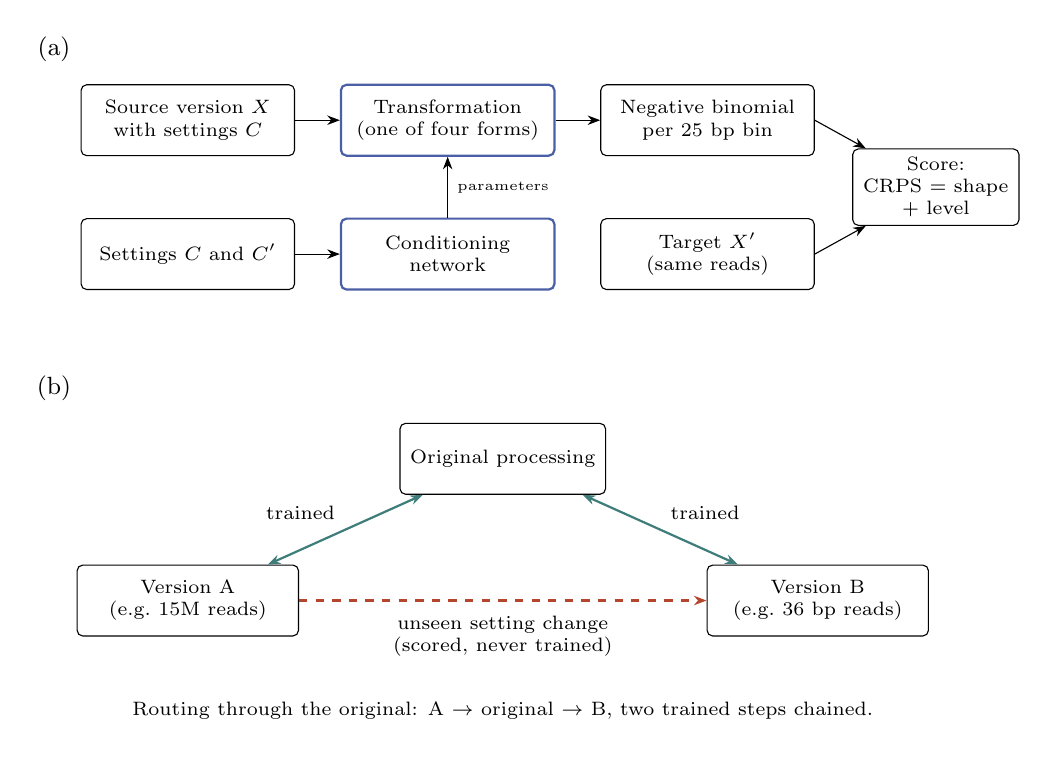
\begin{tikzpicture}[box/.style={draw, rounded corners=2pt, align=center, font=\scriptsize,
    minimum height=0.9cm, text width=2.5cm, inner sep=3pt}, >={Stealth[length=1.6mm]}]
  \node[font=\small] at (-1.7,0.9) {(a)};
  \node[box] (x) at (0,0) {Source version $X$\\ with settings $C$};
  \node[box] (c) at (0,-1.7) {Settings $C$ and $C'$};
  \node[box, draw=dD, thick] (g) at (3.3,-1.7) {Conditioning\\ network};
  \node[box, draw=dD, thick] (f) at (3.3,0) {Transformation\\ (one of four forms)};
  \node[box] (p) at (6.6,0) {Negative binomial\\ per \lit{25}~bp bin};
  \node[box] (t) at (6.6,-1.7) {Target $X'$\\ (same reads)};
  \node[box, text width=1.9cm] (s) at (9.5,-0.85) {Score:\\ CRPS = shape\\ + level};
  \draw[->] (x) -- (f);
  \draw[->] (c) -- (g);
  \draw[->] (g) -- node[right, font=\tiny] {parameters} (f);
  \draw[->] (f) -- (p);
  \draw[->] (p.east) -- (s);
  \draw[->] (t.east) -- (s);
  \begin{scope}[yshift=-4.3cm]
  \node[font=\small] at (-1.7,0.9) {(b)};
  \node[box, text width=2.4cm] (o) at (4.0,0) {Original processing};
  \node[box, text width=2.6cm] (a1) at (0,-1.8) {Version A\\ (e.g.\ \lit{15}M reads)};
  \node[box, text width=2.6cm] (a2) at (8.0,-1.8) {Version B\\ (e.g.\ \lit{36}~bp reads)};
  \draw[<->, thick, gTr] (o) -- node[above left, font=\scriptsize, text=black] {trained} (a1);
  \draw[<->, thick, gTr] (o) -- node[above right, font=\scriptsize, text=black] {trained} (a2);
  \draw[->, thick, dashed, gNv] (a1) -- node[below=2pt, font=\scriptsize, text=black, align=center]
    {unseen setting change\\ (scored, never trained)} (a2);
  \node[font=\scriptsize, align=center] at (4.0,-3.2) {Routing through the original: A $\to$
    original $\to$ B, two trained steps chained.};
  \end{scope}
\end{tikzpicture}
\caption{Design. (a) The correction model. A conditioning network reads the source and target
settings and sets the parameters of a transformation. The transformation turns the source
counts into a negative binomial prediction of the target, which is scored by CRPS against the
real target. (b) Training and scoring pairs within one track. Models train on pairs between
the original processing and each reprocessed version (solid). They are scored also on pairs
between two reprocessed versions (dashed), which they never saw.}\label{fig:design}
\end{figure}

\section{Results and discussion}\label{sec:results}

\subsection{Processing settings change peak heights far more than sampling noise does}\label{sec:r1}

We first measured how far each setting moves a track away from its original processing. Peak
height is the absolute $\log_{\lit{2}}$ fold change of the mean count over the top
\lit{1}\% of bins, on peaks that both versions share. Shape is one minus the Spearman
correlation between the two versions over \lit{1}~kb bins. We compared each change with the
resampling floor at the same depth. Peak height moved beyond the floor in \nPhAbove{} of
\nPh{} setting levels, by \phRatioLo{} to \phRatioHi{} times the floor (Fig.~\ref{fig:peak}).
Depth moved peaks most. At \lit{3.75}M reads, peak height changed by \peakDepthHistLo{} to
\peakDepthHistHi{} $\log_{\lit{2}}$ units in histone marks and by \peakDepthDn{} in DNase-seq.
The antibody-efficiency proxy at \lit{90}\% control reads and the \lit{36}~bp crop came next,
at \peakAbHistLo{} to \peakAbHistHi{} and \peakCropHistLo{} to \peakCropHistHi{} units.
Duplicate removal, the mapping-quality filter and run type moved histone peaks by
\peakRestLo{} to \peakRestHi{} units. Shape, in contrast, moved beyond its floor in only
\nShAbove{} of \nSh{} levels.

For model design, this means that a correction must first get the peak level right. At this
depth, most settings change shape by less than sampling noise does, so a shape score alone
cannot rank them. Each value is a median over the one to three tracks of a mark class and has
no seed variation; the floor's seed range is at most \phFloorSpreadHi{}. A reprocessed version
shares reads with its original, while the floor compares independent halves. A shape change
below the floor is therefore not proof that a setting has no effect. On peaks chosen from the
original alone, depth read about \peakDepthFirstHi{} units in histone marks; the shared peak
set removes this selection bias.

\begin{figure}[t]
\centering
\begin{tikzpicture}
\begin{axis}[base, width=0.95\textwidth, height=6cm, ymode=log, ymin=1e-3, ymax=10,
    xmin=-0.6, xmax=10.6, xtick=data, xticklabels from table={\tblPeak}{lab},
    xticklabel style={rotate=30, anchor=north east}, xtick style={draw=none},
    ylabel={Peak-height change ($\log_{\lit{2}}$ fold)},
    legend style={at={(0.99,0.03)}, anchor=south east}, legend columns=2]
  \addplot[only marks, mark=*, mark size=2pt, color=cNar] table[x=x, y=nar]{\tblPeak};
  \addlegendentry{narrow marks}
  \addplot[only marks, mark=square*, mark size=2pt, color=cBr] table[x=x, y=br]{\tblPeak};
  \addlegendentry{broad marks}
  \addplot[only marks, mark=triangle*, mark size=2.6pt, color=cDn] table[x=x, y=dn]{\tblPeak};
  \addlegendentry{DNase-seq}
  \addplot[only marks, mark=o, mark size=1.8pt, color=black!55] table[x=x, y=fnar]{\tblPeak};
  \addlegendentry{resampling floor}
  \addplot[only marks, mark=o, mark size=1.8pt, color=black!55, forget plot] table[x=x, y=fbr]{\tblPeak};
  \addplot[only marks, mark=o, mark size=1.8pt, color=black!55, forget plot] table[x=x, y=fdn]{\tblPeak};
\end{axis}
\end{tikzpicture}
\caption{Peak-height change caused by each setting level, against the resampling floor. Filled
marks show the median change over the tracks of a mark class, on peaks shared by the original
and the reprocessed version; DNase-seq has no version for some settings. Open grey circles
show the floor, the change between two random halves of the same reads at the same depth. The
y axis is logarithmic. There are no error bars: each value is deterministic, and the floor's
seed range (at most \phFloorSpreadHi{}) is smaller than the marks.}\label{fig:peak}
\end{figure}

\subsection{Most settings act uniformly along the genome, but the mapping-quality filter and read cropping act mainly in hard-to-map regions}\label{sec:r2}

We next asked where along the genome each setting acts. For each setting, we fitted one
monotone map from the original to the reprocessed version over the whole genome. We then took
the $\log_{\lit{2}}$ residual of the reprocessed version in each \lit{1}~kb bin. We first
explained the residual size by signal level, in \lit{40} quantile bins. We then measured the
extra variance explained ($R^{\lit{2}}$) by GC content, mappability, repeat content and peak
context together. A setting that acts uniformly leaves no extra $R^{\lit{2}}$, and one genome-wide
map then corrects it.

Depth acted uniformly. Its mean absolute residual equalled that of the original thinned to
the same depth (\depArm{} against \depNull{} in DNase-seq at \lit{15}M), and the features added
at most \depArmFeatHi{} $R^{\lit{2}}$ against \depNullFeatHi{} for the thinned original.
Duplicate removal and run type in histone marks added at most \dedupFeatHi{}. The
mapping-quality filter at \lit{0} added \mapqZeroLo{} to \mapqZeroHi{}, mostly through
mappability (Fig.~\ref{fig:region}). In the lowest-mappability tenth of bins, its signal was
\mapqZeroDecAllLo{} to \mapqZeroDecAllHi{} $\log_{\lit{2}}$ units above what the genome-wide map
predicted. The \lit{36} and \lit{50}~bp crops added \cropFeatLo{} to \cropFeatHi{}, through
mappability and repeats. A control that permutes the features added at most \knobShufMax{}.

For model design, depth, duplicate removal and run type in histone marks need no positional
input. Read length and the mapping-quality filter need an input that knows the position, such
as a mappability track; Section~\ref{sec:r11} tests this. These readings are exploratory and
come from one to three tracks per class.

\begin{figure}[t]
\centering
\begin{tikzpicture}
\begin{axis}[base, width=0.9\textwidth, height=6cm, ybar, bar width=7pt, ymode=log,
    log origin=infty, ymin=1e-5, ymax=0.5, ylabel={Extra $R^{\lit{2}}$ from regional features},
    xtick=data, xticklabels from table={\tblKnob}{lab}, xtick style={draw=none},
    xticklabel style={rotate=30, anchor=north east}, enlarge x limits=0.06,
    extra y ticks={\knobShufMax}, extra y tick labels={},
    extra y tick style={grid=major, grid style={black, dashed}},
    legend style={at={(0.02,0.98)}, anchor=north west}, area legend]
  \addplot[fill=cNar, draw=none] table[x=x, y=nar]{\tblKnob};
  \addlegendentry{narrow marks}
  \addplot[fill=cBr, draw=none] table[x=x, y=br]{\tblKnob};
  \addlegendentry{broad marks}
\end{axis}
\end{tikzpicture}
\caption{How much regional features explain of each setting's effect. Each bar is the extra
$R^{\lit{2}}$ that GC content, mappability, repeats and peak context add to a signal-level model of
the residual left after one genome-wide map (median over the three tracks of a class). The y
axis is logarithmic. The dashed line is the largest value of a control with permuted features.
There are no error bars, because each value is deterministic.}\label{fig:region}
\end{figure}

\subsection{Sampling noise depends on signal level, not on genomic region}\label{sec:r3}

A correction cannot be more accurate than the resampling floor allows, so we mapped that
floor. We thinned the two random halves of every version along a depth ladder and compared
them bin by bin. At \lit{15}M reads per half, signal level explained \lvlFifteenLo{} to
\lvlFifteenHi{} of the variance of the per-bin disagreement. GC content, mappability, repeats
and peak context together added at most \featMaxFifteen{} (Fig.~\ref{fig:level}a), against
\shufMax{} for permuted features. The \lit{1}~kb shape floor shrank with depth
(Fig.~\ref{fig:level}b). Extrapolated to \lit{30}M reads, it was \shThirtyNar{} for narrow marks,
\shThirtyBr{} for broad marks and \shThirtyDn{} for DNase-seq. Peak height barely moved under
resampling: at most \peakFloorAll{} $\log_{\lit{2}}$ units, even at the lowest depth. Real depth
versions matched the thinned halves (median ratio \realRead{} over \realN{} versions).

For model design, a noise model whose variance depends only on the mean, such as the negative
binomial, describes this floor; a region-specific noise term is not needed. The
\lit{30}M values extrapolate a concave curve, so the histone values may be too high. The seed
range of the floor is at most \shSpreadHi{}.

\begin{figure}[t]
\centering
\begin{tikzpicture}
\begin{axis}[base, name=la, width=0.5\textwidth, height=6cm, ybar, bar width=7pt,
    ymode=log, log origin=infty, ymin=1e-6, ymax=1, ylabel={Variance explained ($R^{\lit{2}}$)},
    xtick=data, xticklabels from table={\tblLevel}{lab}, xtick style={draw=none},
    enlarge x limits=0.25, title={(a) Level against region, \lit{15}M reads per half},
    legend style={at={(0.5,-0.18)}, anchor=north}, legend columns=1, area legend]
  \addplot[fill=pOS, draw=none] table[x=x, y=lvl]{\tblLevel};
  \addlegendentry{signal level}
  \addplot[fill=pSE, draw=none, error bars/.cd, y dir=both, y explicit, error bar style={black}]
    table[x=x, y=feat, y error plus=feathi, y error minus=featlo]{\tblLevel};
  \addlegendentry{extra from four regional features}
  \addplot[fill=black!35, draw=none] table[x=x, y=shuf]{\tblLevel};
  \addlegendentry{extra from permuted features}
\end{axis}
\begin{axis}[base, at={(la.east)}, anchor=west, xshift=1.6cm, width=0.44\textwidth, height=6cm,
    title={(b) Shape floor against depth},
    xlabel={Reads per half (millions)}, ylabel={Shape change, $1-\rho$ on \lit{1}~kb bins},
    xtick={0.907,1.907,2.907,3.907,4.907}, xticklabels={1.9,3.75,7.5,15,30},
    ymin=0, ymax=1, legend style={at={(0.5,-0.3)}, anchor=north}]
  \addplot[color=cNar, mark=*, mark size=1.2pt] table[x=x, y=y]{\tblShReadNar};
  \addlegendentry{narrow marks}
  \addplot[color=cBr, mark=square*, mark size=1.2pt] table[x=x, y=y]{\tblShReadBr};
  \addlegendentry{broad marks}
  \addplot[color=cDn, mark=triangle*, mark size=1.6pt] table[x=x, y=y]{\tblShReadDn};
  \addlegendentry{DNase-seq}
\end{axis}
\end{tikzpicture}
\caption{The resampling floor. (a) Share of the variance of the per-bin disagreement between
two random halves that signal level explains, and the extra share that GC content,
mappability, repeats and peak context add, or that permuted features add (median over
versions; the y axis is logarithmic). Error bars span the smallest to the largest version.
(b) Shape change between the two halves as the halves are thinned; each line is the median
over the versions of a class. The rightmost point (\lit{30}M) is extrapolated. The seed range
(at most \shSpreadHi{}) is smaller than the marks.}\label{fig:level}
\end{figure}

\subsection{Recorded settings help on trained setting changes, but the benefit shrinks on unseen combinations}\label{sec:r4}

We measured the benefit of the settings as the relative CRPS gain of a model over its
shuffled-settings control: the control's CRPS minus the model's, divided by the control's.
Over the \nGenCfg{} configurations, the median gain on counts was \relCntTr{} on trained
setting changes (Fig.~\ref{fig:gen}). It fell to \relCntSame{} on unseen changes within one
setting and to \relCntCross{} on unseen changes that combine two settings. For depth, the gain
fell from \genDepthTr{} to \genDepthSame{}; for read length, from \genCropTr{} to
\genCropSame{}. On the $p$-value track, the gain fell from \relPTr{} to \relPSame{} and
\relPCross{}.

For model design, the settings clearly carry information that the models use. But the models
learn the changes they saw, not a rule that they can apply to new combinations. A model that
claims to correct processing must therefore be tested on unseen setting combinations, not only
on unseen cell types. These readings are exploratory: no threshold was fixed before the runs.

\begin{figure}[t]
\centering
\begin{tikzpicture}
\begin{axis}[base, width=0.85\textwidth, height=6cm, ybar, bar width=9pt, ymin=-0.1, ymax=0.7,
    xtick=data, xticklabels from table={\tblGen}{lab}, xtick style={draw=none},
    xticklabel style={rotate=20, anchor=north east},
    enlarge x limits=0.12, ylabel={Relative CRPS gain over control},
    extra y ticks={0}, extra y tick labels={}, extra y tick style={grid=major, grid style={black, thin}},
    legend style={at={(0.98,0.98)}, anchor=north east}, legend columns=1, area legend]
  \addplot[fill=gTr, draw=none, error bars/.cd, y dir=both, y explicit]
    table[x=x, y=tr, y error plus=trhi, y error minus=trlo]{\tblGen};
  \addlegendentry{trained changes}
  \addplot[fill=gNv, draw=none, error bars/.cd, y dir=both, y explicit]
    table[x=x, y=sa, y error plus=sahi, y error minus=salo]{\tblGen};
  \addlegendentry{unseen, one setting}
  \addplot[fill=gCr, draw=none, error bars/.cd, y dir=both, y explicit]
    table[x=x, y=cr, y error plus=crhi, y error minus=crlo]{\tblGen};
  \addlegendentry{unseen, two settings}
\end{axis}
\end{tikzpicture}
\caption{Benefit of the recorded settings on trained and unseen setting changes, in counts.
Each bar is the median, over the \nGenCfg{} model configurations, of the relative CRPS gain of
the model over its shuffled-settings control. Error bars span the \lit{25}th to the \lit{75}th percentile
over configurations. Per setting, only changes within one setting exist; duplicate removal and
run type have one level and so no unseen change of their own.}\label{fig:gen}
\end{figure}

\subsection{The failure to transfer is not a lack of capacity}\label{sec:r5}

Depth gives an exact test of transfer, because the real versions obeyed the depth rule within
\lawData\%. On trained depth changes, every model followed the rule closely: the error was
\ruleTrLo{} to \ruleTrHi{} over all eight form-and-input combinations and both training scopes
(Fig.~\ref{fig:rule}a). On unseen depth changes, the error rose to \ruleNeverLo{} to
\ruleNeverHi{}. Chaining two trained steps through the original processing brought it back to
\ruleViaLo{} to \ruleViaHi{}. We then tried five fixes on the CNN or the affine form: removing
the pseudocount from the log transform, a Poisson loss on the mean, a four times wider
conditioning network, a twice wider transformation and an encoder--decoder design. All of them
kept the trained error low (\fixTrLo{} to \fixTrHi{}) and left the unseen error at \fixNeverLo{}
to \fixNeverHi{} (Fig.~\ref{fig:rule}b).

We also tried a closed-form depth offset. It removes the source depth before the
transformation and adds the target depth after it. The offset helped only the affine form: its
DNase CRPS fell from \oldA{} $\pm$ \oldAw{} (\oldAOS{} shape + \oldASE{} level) to \offA{}
$\pm$ \offAw{} (\offAOS{} + \offASE{}), against a threshold of \offBar{}. The other forms improved
significantly in \offBDclear{} of \offBDn{} cells. Even with the offset, no model met the depth
rule within \lit{0.10} in any of \offLawN{} cells. The shuffled-settings controls of the CNN came
much closer (\offTwinLo{} to \offTwinHi{}), because the network bends the exact rule when it can
read the depth settings.

For model design, the transfer failure is a failure to generalise, not a shortage of capacity.
A next model should impose known physical rules, such as depth scaling, rather than learn them,
and should check them on unseen changes. These readings are exploratory, and their thresholds
were set after the runs.

\begin{figure}[t]
\centering
\begin{tikzpicture}
\begin{axis}[base, name=ra, width=0.42\textwidth, height=6cm, ymin=0, ymax=0.7,
    xmin=-0.5, xmax=3.5, xtick=data, xticklabels from table={\tblRule}{lab}, xtick style={draw=none},
    xticklabel style={rotate=30, anchor=north east},
    ylabel={Depth-rule error ($|\log_{\lit{2}}|$)}, title={(a) Model forms, one model per track},
    legend style={at={(0.02,0.98)}, anchor=north west}]
  \addplot[only marks, mark=o, mark size=2.2pt, color=gTr, thick] table[x=x, y=tr]{\tblRule};
  \addlegendentry{trained changes}
  \addplot[only marks, mark=*, mark size=2.2pt, color=gNv] table[x=x, y=nv]{\tblRule};
  \addlegendentry{unseen changes}
  \addplot[only marks, mark=diamond*, mark size=2.6pt, color=dD] table[x=x, y=via]{\tblRule};
  \addlegendentry{unseen, via original}
\end{axis}
\begin{axis}[base, at={(ra.east)}, anchor=west, xshift=3.6cm, width=0.38\textwidth, height=6cm,
    xmin=0, xmax=0.75, ymin=-0.6, ymax=4.6, ytick=data, yticklabels from table={\tblFix}{lab},
    xlabel={Depth-rule error ($|\log_{\lit{2}}|$)}, title={(b) Attempted fixes},
    legend style={at={(0.5,-0.3)}, anchor=north}, legend columns=2]
  \addplot[only marks, mark=*, mark size=2.2pt, color=gNv, error bars/.cd, x dir=both, x explicit]
    table[x=nv, y=y, x error=e]{\tblFix};
  \addlegendentry{unseen changes}
  \addplot[only marks, mark=o, mark size=2.2pt, color=gTr, thick] table[x=tr, y=y]{\tblFix};
  \addlegendentry{trained changes}
\end{axis}
\end{tikzpicture}
\caption{The depth rule on trained and unseen depth changes. The error is the median absolute
$\log_{\lit{2}}$ difference between the predicted and the true ratio of total counts; zero means the
rule is met. (a) The four transformation forms, each trained as one model per track (median
over \lit{3} seeds). Diamonds chain two trained steps through the original processing. (b)
Five attempted fixes; error bars on the unseen values span the seed range.}\label{fig:rule}
\end{figure}

\subsection{A per-bin monotone curve captures most of the correction, and a convolutional network adds little}\label{sec:r6}

On trained depth changes, the monotone curve, the kernel-plus-curve form and the CNN closed
\gcBDLo{} to \gcBDHi{} of the gap between the covariate-free monotone baseline and the depth
oracle in every mark class (Fig.~\ref{fig:forms}a). Their gain over the baseline was
significant in \nBDgain{} of \nBDcells{} cells. The affine form did not close the gap
(\gcALo{} to \gcAHi{} in DNase-seq and narrow marks). Over all settings, we compared each form
in \nCellsB{} count cells, one per mark class, training scope and bin set (all bins or the top
\lit{1}\%). The affine form beat its shuffled-settings control in \nTwA{} cells, and the other
three forms in \nTwB{}, \nTwC{} and \nTwD{} (Fig.~\ref{fig:forms}b). Each step up in capacity
paid less. The curve beat the affine form in \nBlB{} cells, the kernel beat the curve in
\nBlC{}, and the CNN beat the kernel in \nBlD{}. In DNase-seq, the per-track CRPS was \dnA{}
$\pm$ \dnAS{} for the affine form (\dnAOS{} + \dnASE{}), \dnB{} $\pm$ \dnBS{} for the curve
(\dnBOS{} + \dnBSE{}), \dnC{} $\pm$ \dnCS{} for the kernel (\dnCOS{} + \dnCSE{}) and \dnD{} $\pm$
\dnDS{} for the CNN (\dnDOS{} + \dnDSE{}). Most of the affine form's error is in the level part.

For model design, the correction module can be small. A per-bin monotone curve, conditioned
on the settings, is a sufficient first design for count data. These readings are exploratory,
and the depth oracle was redefined after the run.

\begin{figure}[t]
\centering
\begin{tikzpicture}
\begin{axis}[base, name=fa, width=0.5\textwidth, height=6cm, ymin=-2.2, ymax=1.6,
    xmin=-0.5, xmax=2.5, xtick={0,1,2}, xticklabels={DNase-seq, narrow, broad},
    xtick style={draw=none}, ylabel={Gap closed}, title={(a) Depth, trained changes},
    extra y ticks={0,0.5}, extra y tick labels={}, extra y tick style={grid=major, grid style={black!40, thin}},
    legend style={at={(0.5,-0.17)}, anchor=north}, legend columns=4]
  \addplot[only marks, mark=*, mark size=1.8pt, color=dA, error bars/.cd, y dir=both, y explicit]
    table[x=x, y=gc, y error=err]{\tblGapA};
  \addlegendentry{affine}
  \addplot[only marks, mark=*, mark size=1.8pt, color=dB, error bars/.cd, y dir=both, y explicit]
    table[x=x, y=gc, y error=err]{\tblGapB};
  \addlegendentry{monotone}
  \addplot[only marks, mark=*, mark size=1.8pt, color=dC, error bars/.cd, y dir=both, y explicit]
    table[x=x, y=gc, y error=err]{\tblGapC};
  \addlegendentry{kernel + curve}
  \addplot[only marks, mark=*, mark size=1.8pt, color=dD, error bars/.cd, y dir=both, y explicit]
    table[x=x, y=gc, y error=err]{\tblGapD};
  \addlegendentry{CNN}
\end{axis}
\begin{axis}[base, at={(fa.east)}, anchor=west, xshift=1.6cm, width=0.44\textwidth, height=6cm,
    ybar, bar width=9pt, ymin=0, ymax=12.5, xtick=data, xticklabels from table={\tblWins}{lab},
    xtick style={draw=none}, xticklabel style={rotate=30, anchor=north east},
    enlarge x limits=0.18, ylabel={Count cells won (of \lit{12})},
    title={(b) All settings, trained changes},
    legend style={at={(0.5,-0.32)}, anchor=north}, legend columns=1, area legend]
  \addplot[fill=gTr, draw=none] table[x=x, y=tw]{\tblWins};
  \addlegendentry{beats shuffled-settings control}
  \addplot[fill=gCr, draw=none] table[x=x, y=bl]{\tblWins};
  \addlegendentry{beats the next simpler form}
\end{axis}
\end{tikzpicture}
\caption{Capacity of the transformation. (a) Fraction of the gap from the covariate-free
monotone baseline to the depth oracle that each form closes, from original to reprocessed
version, one model per track; \lit{1} means the oracle is reached. Each error bar extends \lit{2} times
the seed range, in gap units, on each side. Grid lines mark zero and \lit{0.5}. (b) Number of count cells, out
of \lit{12}, in which each form beats its shuffled-settings control, and beats the form one
step below it, by more than \lit{2} times the seed range.}\label{fig:forms}
\end{figure}

\subsection{Training on pairs between two reprocessed versions teaches the depth ratio, not the distribution}\label{sec:r7}

If the models fail on unseen changes only because they never saw a pair between two
reprocessed versions, adding such pairs should fix it. We tested this in a pre-registered
experiment with the per-track CNN. We held out the \lit{7.5}M depth version entirely and added
the two pairs between the \lit{15}M and \lit{3.75}M versions to training. We scored all pairs
that involve the held-out version. Each check had to close at least half (\lit{0.5}) of the gap
between the direct route and the route through the original processing.

The depth rule passed. Its error was \armOneRule{} (seed range \armOneRuleS{}), against
\armRefRule{} for the direct route and \armViaRule{} through the original, so the added pairs
closed \cOneGap{} of the gap (Fig.~\ref{fig:arm}b). CRPS failed. It was \crArm{} (\crArmOS{}
shape + \crArmSE{} level, seed range \crArmS{}), against \crRef{} (\crRefOS{} + \crRefSE{}) direct
and \crVia{} (\crViaOS{} + \crViaSE{}) through the original (Fig.~\ref{fig:arm}a). The gap closed
was \cFourGap{}, and the gain over the direct route was \cFourGainChk{} against a required
\cFourBar{}. The loss sits in the level part. After the test, we also read a version trained on
every pair between reprocessed versions that avoids \lit{7.5}M. It reached \crArmTwo{}
(\crArmTwoOS{} + \crArmTwoSE{}), close to the route through the original.

For model design, a few counterfactual pairs teach the size of a setting's effect but not the
full distribution; dense pairs may be needed. DNase-seq drives the CRPS failure, the depth-rule
pass varies across seeds (\lawSeedLo{} to \lawSeedHi{}), and the dense-pair result was read
after the run on one held-out level.

\begin{figure}[t]
\centering
\begin{tikzpicture}
\begin{axis}[stk, name=aa, width=0.5\textwidth, height=6cm, ymax=0.75,
    xticklabels from table={\tblArm}{lab}, enlarge x limits=0.18, ylabel={CRPS},
    title={(a) CRPS, held-out pairs}]
  \addplot[fill=pOS, draw=none] table[x=x, y=os]{\tblArm};
  \addlegendentry{shape}
  \addplot[fill=pSE, draw=none, error bars/.cd, y dir=both, y explicit, error bar style={black}]
    table[x=x, y=se, y error=err]{\tblArm};
  \addlegendentry{level}
\end{axis}
\begin{axis}[base, at={(aa.east)}, anchor=west, xshift=1.6cm, width=0.44\textwidth, height=6cm,
    ymin=0, ymax=0.35, xmin=-0.5, xmax=3.5, xtick=data, xticklabels from table={\tblArm}{lab},
    xticklabel style={rotate=30, anchor=north east, font=\scriptsize}, xtick style={draw=none},
    ylabel={Depth-rule error ($|\log_{\lit{2}}|$)}, title={(b) Depth rule, held-out pairs}]
  \addplot[only marks, mark=*, mark size=2.2pt, color=dD, error bars/.cd, y dir=both, y explicit]
    table[x=x, y=rule, y error=rerr]{\tblArm};
\end{axis}
\end{tikzpicture}
\caption{Adding pairs between reprocessed versions to training (per-track CNN). From left: the
direct route, the route through the original processing, training with one added pair of
depth versions, and training with all such pairs. (a) CRPS on held-out pairs, split into shape
(blue) and level (gold). (b) Depth-rule error. Error bars span the seed range over \lit{3}
seeds.}\label{fig:arm}
\end{figure}

\subsection{Routing through the original processing helps a per-track model but not a model shared across tracks}\label{sec:r8}

Another way to reach an unseen change is to chain two trained steps: from the source version
to the original processing, then from the original to the target version. For one model per
track, this route lowered CRPS on unseen changes from \ptDir{} (\ptDirOS{} + \ptDirSE{}, seed
range \ptDirS{}) to \ptVia{} (\ptViaOS{} + \ptViaSE{}, \ptViaS{}). The gain of \ptGain{} exceeded
the threshold of \ptBar{} (Fig.~\ref{fig:route}). The route also met the depth rule (\ptRuleVia{}
against \ptRuleDir{} direct).

We then pre-registered the same test for one model shared across all seven tracks, with
\lit{6} seeds. Routing had to win significantly in two thirds of the \nCells{} cells, one cell
per pair of source and target setting. It won in \nCellWin{} and lost in \nCellWorse{}. Pooled
over cells, routing was lower in \nSeedPos{} of \nSeedAll{} seeds. The pooled gain of \pGain{}
(direct \pDir{} = \pDirOS{} + \pDirSE{}; routed \pCh{} = \pChOS{} + \pChSE{}) was still below
the threshold of \pGainBar{}, because the routed seed range was \pChS{}. The routed shared model
did meet the depth rule (\pLawCh{} against a pre-registered limit of \lit{0.16}). In an
unplanned reading, a shared model trained with an agreement loss between the two routes
scored \pAg{} (\pAgOS{} + \pAgSE{}) on the direct route. Its gain of \pAgGain{} just exceeded
the threshold of \pAgBar{}.

For model design, routing through a reference version is not a general fix for a shared model,
and the agreement loss is only an exploratory lead. The control on trained pairs missed its
band on six seeds (\nOneGap{} against \nOneBar{}); we counted it on the three seeds shared with
the reference model, a decision made after the run. The per-track result was read after its
run.

\begin{figure}[t]
\centering
\begin{tikzpicture}
\begin{axis}[stk, width=0.8\textwidth, height=6cm, ymax=0.85, xmin=-0.6, xmax=5.1,
    xticklabels from table={\tblRoute}{lab}, ylabel={CRPS, unseen changes}]
  \addplot[fill=pOS, draw=none] table[x=x, y=os]{\tblRoute};
  \addlegendentry{shape}
  \addplot[fill=pSE, draw=none, error bars/.cd, y dir=both, y explicit, error bar style={black}]
    table[x=x, y=se, y error=err]{\tblRoute};
  \addlegendentry{level}
\end{axis}
\end{tikzpicture}
\caption{Routing through the original processing. CRPS on unseen setting changes, split into
shape (blue) and level (gold), for one model per track (left pair, \lit{3} seeds) and one model
shared across tracks (right three bars, \lit{6} seeds). The last bar is the shared model
trained with an agreement loss between the direct and the routed prediction. Error bars span
the seed range.}\label{fig:route}
\end{figure}

\subsection{Predicting counts and deriving \texorpdfstring{$p$}{p}-values with the peak caller's formula works almost as well as learning the map}\label{sec:r9}

The challenge scored $-\log_{\lit{10}} p$-value tracks, so a model must also produce them. We
compared maps from a count distribution and its matched control to the peak caller's $p$-value
track, first on the true counts of the narrow-mark versions of one track. We scored them by
CRPS on $\log(\lit{1}+p)$, which we call log CRPS. The peak caller's own fragment-window formula
scored \pFrag{} (\pFragOS{} + \pFragSE{}). The best learned map, the formula plus a small
correction network, scored \pFm{} $\pm$ \pFmS{} (\pFmOS{} + \pFmSE{}). A learned network alone
scored \pMlp{}, and an affine map \pAff{} (Fig.~\ref{fig:pmap}).

Fed the CNN's predicted counts, every derived map scored a CRPS of \pChainLo{} to \pChainHi{} on
the $p$-value track. A model that predicts $p$-values directly scored \pOldD{}. No derived
prediction diverged (CRPS above \lit{20}), whereas the direct $p$-value output of the CNN
reached a mean DNase CRPS of \pDirectDnD{}. A next model should therefore predict counts and
derive $p$-values by the formula; the remaining error then belongs to the count model. These
results come from one track and one seed of the count model.

\begin{figure}[t]
\centering
\begin{tikzpicture}
\begin{axis}[stk, width=0.7\textwidth, height=6cm, ymax=0.2,
    yticklabel style={/pgf/number format/fixed, /pgf/number format/precision=2},
    xticklabels from table={\tblPmap}{lab}, enlarge x limits=0.15, ylabel={Log CRPS}]
  \addplot[fill=pOS, draw=none] table[x=x, y=os]{\tblPmap};
  \addlegendentry{shape}
  \addplot[fill=pSE, draw=none, error bars/.cd, y dir=both, y explicit, error bar style={black}]
    table[x=x, y=se, y error=err]{\tblPmap};
  \addlegendentry{level}
\end{axis}
\end{tikzpicture}
\caption{From true counts to the $p$-value track (narrow marks, one track). Each bar is the
log CRPS of a map, split into shape (blue) and level (gold). The two formulas have no seed;
error bars on the learned maps span the seed range over \lit{3} seeds.}\label{fig:pmap}
\end{figure}

\subsection{Adding an imputation objective does not change transfer at this scale}\label{sec:r10}

CANDI trains its correction jointly with imputation, so the negative results above might not
hold there. We pre-registered a test on the shared model. A cross-assay objective predicted
another assay of the same cell type from the original version. A denoising objective
reconstructed masked bins. At weight \lit{1}, cross-assay training moved CRPS on unseen changes
by \jXd{} (threshold \jXdBar{}) and denoising by \jDnd{} (threshold \jDndBar{}). Neither change
was significant (Fig.~\ref{fig:joint}). Correction alone scored \jAlone{} (\jAloneOS{} +
\jAloneSE{}, seed range \jAloneS{}), and cross-assay training \jX{} (\jXOS{} + \jXSE{}, \jXS{}).
At weight \lit{4}, cross-assay training came close (\jXfourd{} against \jXfourdBar{}), mostly
in the level part (\jXfourdSE{}). Both joint models beat their shuffled-settings controls on
unseen changes, by \jXtw{} and \jDntw{}.

For model design, the earlier negative results on model form probably carry over to joint
training at this scale. The trend at weight \lit{4} suggests that a stronger imputation term may
improve the level. The power of the test was \powJoint\%. Its planned check against the
shuffled-settings control on trained pairs could not fail as built, because the control was
scored on its own training labels.

\begin{figure}[t]
\centering
\begin{tikzpicture}
\begin{axis}[stk, width=0.8\textwidth, height=6cm, ymax=1.15,
    xticklabels from table={\tblJoint}{lab}, enlarge x limits=0.08, ylabel={CRPS, unseen changes}]
  \addplot[fill=pOS, draw=none] table[x=x, y=os]{\tblJoint};
  \addlegendentry{shape}
  \addplot[fill=pSE, draw=none, error bars/.cd, y dir=both, y explicit, error bar style={black}]
    table[x=x, y=se, y error=err]{\tblJoint};
  \addlegendentry{level}
\end{axis}
\end{tikzpicture}
\caption{An added imputation objective, one model shared across tracks. CRPS on unseen
setting changes, split into shape (blue) and level (gold), for correction alone, correction
with its loss rescaled to match the joint loss, the two joint objectives at weight \lit{1}
(cross-assay also at weight \lit{4}) and their shuffled-settings controls. Error bars span the
seed range over \lit{3} seeds.}\label{fig:joint}
\end{figure}

\subsection{A mappability input improves correction in hard-to-map regions}\label{sec:r11}

Section~\ref{sec:r2} showed that read cropping and the mapping-quality filter act through
mappability. We pre-registered adding per-bin \lit{36}-mer mappability as an extra input channel
to the shared model. We scored the lowest-mappability tenth of \lit{1}~kb blocks. There, the
input lowered CRPS on all \nMapLPass{} of \nMapTracks{} tracks for the \lit{36}~bp crop: \mMapL{}
(\mMapLOS{} + \mMapLSE{}) against \mAlL{} (\mAlLOS{} + \mAlLSE{}) without it
(Fig.~\ref{fig:map}). It did the same on all \nMapQPass{} tracks for the mapping-quality filter at
\lit{0}: \mMapQ{} (\mMapQOS{} + \mMapQSE{}) against \mAlQ{} (\mAlQOS{} + \mAlQSE{}). Mappability
shifted by \lit{5}~Mb, which keeps the input's distribution but breaks its alignment, did much
worse. The aligned input beat it by \sMapQ{} (threshold \sMapQBar{}) for the filter and by
\sMapL{} (threshold \sMapLBar{}) for the crop. The gain stayed local: genome-wide CRPS was
\gMap{} with the input and \gAl{} without it. One-hot DNA sequence as input recovered
\dnaShareLo{} to \dnaShareHi{} of the mappability gain.

For model design, a mappability channel belongs in the first stage of the next model. The
evidence is weak, because a pre-registered control failed: CRPS on the depth versions, which
should not change, changed by \mDepthChg{} against a seed standard deviation of \mDepthSD{}.
DNase-seq has no crop version, so six tracks were scored instead of seven. The power of the
test was \powMap\%.

\begin{figure}[t]
\centering
\begin{tikzpicture}
\begin{axis}[stk, width=0.85\textwidth, height=6cm, ymax=0.75,
    xticklabels from table={\tblMap}{lab}, enlarge x limits=0.06, ylabel={CRPS, lowest-mappability tenth}]
  \addplot[fill=pOS, draw=none] table[x=x, y=os]{\tblMap};
  \addlegendentry{shape}
  \addplot[fill=pSE, draw=none, error bars/.cd, y dir=both, y explicit, error bar style={black}]
    table[x=x, y=se, y error=err]{\tblMap};
  \addlegendentry{level}
\end{axis}
\end{tikzpicture}
\caption{A mappability input, one model shared across tracks. CRPS in the lowest-mappability
tenth of \lit{1}~kb blocks on the \lit{36}~bp crop (left four) and the mapping-quality filter
at \lit{0} (right four), split into shape (blue) and level (gold), as the mean over tracks.
Inputs: none, aligned mappability, mappability shifted by \lit{5}~Mb, and one-hot DNA sequence.
Error bars span the seed range over \lit{3} seeds.}\label{fig:map}
\end{figure}

\subsection{CANDI's current training corpus can teach only depth, and run type has no paired examples}\label{sec:r12}

CANDI's two corpora hold processed signal only: \corpEic{} challenge experiments and
\corpMerged{} merged tracks, all built from released signal files. Random thinning of counts can
make depth pairs from them, but it cannot make a pair for any other setting. On the \nPanelAssays{}-assay
panel that CANDI trains on, assay and read length fully determine run type: the conditional
entropy of run type is \bitsPanel{} bits, against \bitsFull{} bits on the full challenge panel.
The model therefore cannot learn run type, the setting behind the challenge's failure, from
this panel.

We also probed a trained CANDI model directly. We kept its input fixed and changed only the
output-side read length or run type to the value of a reprocessed version, on \lit{chr21}. Told
\lit{36}~bp reads, it moved its predicted level by \swLPredLo{} to \swLPredHi{} $\log_{\lit{2}}$
units. The real versions moved by \swLRealLo{} to \swLRealHi{}, mostly because shorter reads
cover fewer bins. Told paired-end, it moved histone predictions by \swPPredLo{} to \swPPredHi{}
(real \swPRealLo{} to \swPRealHi{}) and the DNase prediction by \swDPredLo{} to \swDPredHi{} (real
\swDRealLo{}; Fig.~\ref{fig:candi}).

For model design, CANDI uses both settings, but not in the direction the real data move. Other
settings need new paired data, and read-level settings need the pipeline rerun from raw reads
(median \costFastq{} hours per version). The probe failed its own controls in all three runs:
its depth control failed, and its reproducibility test could not separate a real per-bin
effect from pure thinning. We therefore read only the level over the whole chromosome; whether
CANDI tracks the per-region pattern is unknown.

\begin{figure}[t]
\centering
\begin{tikzpicture}
\begin{axis}[base, width=0.6\textwidth, height=6.4cm,
    xmin=-1.3, xmax=0.9, ymin=-1.3, ymax=0.9,
    xlabel={Real level change ($\log_{\lit{2}}$)}, ylabel={Predicted level change ($\log_{\lit{2}}$)},
    legend style={at={(0.5,-0.2)}, anchor=north}]
  \addplot[gray, dashed, domain=-1.3:0.9, forget plot] {x};
  \addplot[only marks, mark=*, mark size=1.8pt, color=cNar] table[x=x, y=y]{\tblSwL};
  \addlegendentry{told \lit{36}~bp reads}
  \addplot[only marks, mark=square*, mark size=1.8pt, color=cBr] table[x=x, y=y]{\tblSwP};
  \addlegendentry{told paired-end, histone}
  \addplot[only marks, mark=triangle*, mark size=2.2pt, color=cDn] table[x=x, y=y]{\tblSwD};
  \addlegendentry{told paired-end, DNase-seq}
\end{axis}
\end{tikzpicture}
\caption{A trained CANDI model told a reprocessed version's read length or run type. Each
point is one track and one of \lit{2} model seeds: the change in predicted level over
\lit{chr21} against the real change between the original and the reprocessed version. The
dashed line marks agreement. There are no error bars; the two seeds of each track are shown as
separate points.}\label{fig:candi}
\end{figure}

\section{Conclusion}\label{sec:conclusion}

The recorded processing settings carry real information. On setting changes seen in training,
models that read them beat a shuffled-settings control, and a per-bin monotone curve captures
most of the correction. On unseen combinations of settings, this benefit largely disappears,
and no model reproduces the exact depth rule. More capacity, other losses, an added
imputation objective and a shared route through the original processing did not change this.
The answer to our question is therefore partial: the settings suffice for changes a model has
seen, but the models tested here do not learn a correction that transfers. This reading would be
settled by a pre-registered transfer test on more tracks.

Several lessons carry over to the next model. It should predict counts with a negative
binomial output and derive $p$-values by the peak caller's formula. Its correction module can
be a small monotone curve per bin. It should impose depth scaling as a fixed rule, or at least
use the depth rule as a check. It should take a mappability input. It should be judged against
a shuffled-settings control, beyond twice the seed range, on unseen setting combinations.

\paragraph{Limitations.} The testbed has seven tracks and three to six seeds per model. Most
results are exploratory, with thresholds set after the data were seen. The pre-registered tests
had a joint power of only \powJoint\% to \powPivot\%. The depth oracle was redefined after its
run, and no exact reference prediction exists for run type. The $p$-value maps rest on one track. Finally, the
correction was trained on its own, so its failures may not hold inside a full imputation model.

\paragraph{Next steps.} We list the options without ranking them.
\begin{itemize}
\item \textbf{A first small prototype} with depth and a mappability channel, judged by the
shuffled-settings control, the seed range and the depth rule on unseen changes. It costs a
testbed-scale run (\costTrLo{} to \costTrHi{} minutes of training per model). It would teach
whether correction survives inside an imputation model.
\item \textbf{A pre-registered test of the agreement loss}, with \lit{6} seeds. It costs one
testbed-scale run. It would teach whether the exploratory lead in Section~\ref{sec:r8} is real.
\item \textbf{A closed-form depth offset with depth hidden from the network}. It costs a rerun
of the offset experiment. It would teach whether imposing the rule removes the depth failure.
\item \textbf{The run-type effect on more tracks}, from challenge test tracks reprocessed as
single-end. It costs CPU-only analysis if suitable products exist. It would teach how large the
challenge's failure cause is for each assay.
\item \textbf{New paired versions for CANDI's corpus.} Read-level settings need the pipeline
rerun from raw reads (median \costFastq{} hours per version; about \costBam{} hour for settings
applied after alignment). It would teach whether real pairs fix transfer at scale.
\end{itemize}

\backmatter
\bibliography{references}

\end{document}
